%%==================================================
%% diss.tex for SJTU Master Thesis
%% based on CASthesis
%% modified by wei.jianwen@gmail.com
%% version: 0.3a
%% Encoding: UTF-8
%% last update: Dec 5th, 2010
%%==================================================

% 字号选项: c5size 五号(默认) cs4size 小四
% 双面打印(注意字号设置)
\documentclass[cs4size, a4paper, twoside]{sjtuthesis} 
% 单面打印(注意字号设置)
% \documentclass[cs4size, a4paper, oneside, openany]{sjtuthesis} 


% \usepackage[sectionbib]{chapterbib}%每章都用参考文献

\newboolean{DOIT}
\setboolean{DOIT}{false}%编译某些只想自己看的内容,编译true,否则false

%% 行距缩放因子(x倍字号)
\renewcommand{\baselinestretch}{1.3}

% 设置图形文件的搜索路径
\graphicspath{{figure/}{figures/}{logo/}{logos/}{graph/}{graphs}}

%%========================================
%% 在sjtuthesis.cls中定义的有用命令
%%========================================
% \cndash 中文破折号
% 数学常量
% \me 对数常数e
% \mi 虚数单位i
% \mj 虚数单位j
% \dif 直立的微分算符d为直立体。
% 可伸长的数学箭头、等号
% \myRightarrow{}{}
% \myLeftarrow{}{}
% \myBioarrow{}{}
% \myLongEqual{}{}
% 参考文献
% \upcite{} 上标引用
%%========================================


\begin{document}

%%%%%%%%%%%%%%%%%%%%%%%%%%%%%% 
%% 封面
%%%%%%%%%%%%%%%%%%%%%%%%%%%%%% 

% 中文封面内容(关注内容而不是形式)
\title{基于内存计算的文件系统的研究和应用}
\author{朱\quad{}佳顺}
\advisor{黄林鹏教授}
\degree{学士}
\defenddate{2014年1月16日}
\school{上海交通大学}
\institute{电子信息与电气工程学院}
\studentnumber{5100109194}
\major{计算机科学与技术}

% 英文封面内容(关注内容而不是表现形式)
\englishtitle{The research and application of file system based on memory computing}
\englishauthor{\textsc{Jiashun Zhu}}
\englishadvisor{Prof. \textsc{Linpeng Huang}}
\englishschool{Shanghai Jiao Tong University}
\englishinstitute{\textsc{Depart of computer science and engineering} \\
  \textsc{Shanghai Jiao Tong University} \\
  \textsc{Shanghai, P.R.China}}
\englishdegree{Bachelor}
\englishmajor{Computer Science}
%\englishdate{Jun, 2014}

% 封面
\maketitle

% 英文封面
\makeenglishtitle

% 论文原创性声明和使用授权
\makeDeclareOriginal
\makeDeclareAuthorization

%%%%%%%%%%%%%%%%%%%%%%%%%%%%%% 
%% 前言
%%%%%%%%%%%%%%%%%%%%%%%%%%%%%% 
\frontmatter

% 摘要
%%==================================================
%% abstract.tex for SJTU Master Thesis
%% based on CASthesis
%% modified by wei.jianwen@gmail.com
%% version: 0.3a
%% Encoding: UTF-8
%% last update: Dec 5th, 2010
%%==================================================

\begin{abstract}

  上海交通大学是我国历史最悠久的高等学府之一,是教育部直属、教育部与上海市共建的全国重点大学,是国家 “七五”、“八五”重点建设和“211工程”、“985工程”的首批建设高校。经过115年的不懈努力,上海交通大学已经成为一所“综合性、研究型、国际化”的国内一流、国际知名大学,并正在向世界一流大学稳步迈进。 

 十九世纪末,甲午战败,民族危难。中国近代著名实业家、教育家盛宣怀和一批有识之士秉持“自强首在储才,储才必先兴学”的信念,于1896年在上海创办了交通大学的前身——南洋公学。建校伊始,学校即坚持“求实学,务实业”的宗旨,以培养“第一等人才”为教育目标,精勤进取,笃行不倦,在二十世纪二三十年代已成为国内著名的高等学府,被誉为“东方MIT”。抗战时期,广大师生历尽艰难,移转租界,内迁重庆,坚持办学,不少学生投笔从戎,浴血沙场。解放前夕,广大师生积极投身民主革命,学校被誉为“民主堡垒”。

 新中国成立初期,为配合国家经济建设的需要,学校调整出相当一部分优势专业、师资设备,支持国内兄弟院校的发展。五十年代中期,学校又响应国家建设大西北的号召,根据国务院决定,部分迁往西安,分为交通大学上海部分和西安部分。1959年3月两部分同时被列为全国重点大学,7月经国务院批准分别独立建制,交通大学上海部分启用“上海交通大学”校名。历经西迁、两地办学、独立办学等变迁,为构建新中国的高等教育体系,促进社会主义建设做出了重要贡献。六七十年代,学校先后归属国防科工委和六机部领导,积极投身国防人才培养和国防科研,为“两弹一星”和国防现代化做出了巨大贡献。

   改革开放以来,学校以“敢为天下先”的精神,大胆推进改革:率先组成教授代表团访问美国,率先实行校内管理体制改革,率先接受海外友人巨资捐赠等,有力地推动了学校的教学科研改革。1984年,邓小平同志亲切接见了学校领导和师生代表,对学校的各项改革给予了充分肯定。在国家和上海市的大力支持下,学校以“上水平、创一流”为目标,以学科建设为龙头,先后恢复和兴建了理科、管理学科、生命学科、法学和人文学科等。1999年,上海农学院并入;2005年,与上海第二医科大学强强合并。至此,学校完成了综合性大学的学科布局。近年来,通过国家“985工程”和“211工程”的建设,学校高层次人才日渐汇聚,科研实力快速提升,实现了向研究型大学的转变。与此同时,学校通过与美国密西根大学等世界一流大学的合作办学,实施国际化战略取得重要突破。1985年开始闵行校区建设,历经20多年,已基本建设成设施完善,环境优美的现代化大学校园,并已完成了办学重心向闵行校区的转移。学校现有徐汇、闵行、法华、七宝和重庆南路(卢湾)5个校区,总占地面积4840亩。通过一系列的改革和建设,学校的各项办学指标大幅度上升,实现了跨越式发展,整体实力显著增强,为建设世界一流大学奠定了坚实的基础。

  交通大学始终把人才培养作为办学的根本任务。一百多年来,学校为国家和社会培养了20余万各类优秀人才,包括一批杰出的政治家、科学家、社会活动家、实业家、工程技术专家和医学专家,如江泽民、陆定一、丁关根、汪道涵、钱学森、吴文俊、徐光宪、张光斗、黄炎培、邵力子、李叔同、蔡锷、邹韬奋、陈敏章、王振义、陈竺等。在中国科学院、中国工程院院士中,有200余位交大校友;在国家23位“两弹一星”功臣中,有6位交大校友;在18位国家最高科学技术奖获得者中,有3位来自交大。交大创造了中国近现代发展史上的诸多“第一”:中国最早的内燃机、最早的电机、最早的中文打字机等;新中国第一艘万吨轮、第一艘核潜艇、第一艘气垫船、第一艘水翼艇、自主设计的第一代战斗机、第一枚运载火箭、第一颗人造卫星、第一例心脏二尖瓣分离术、第一例成功移植同种原位肝手术、第一例成功抢救大面积烧伤病人手术等,都凝聚着交大师生和校友的心血智慧。改革开放以来,一批年轻的校友已在世界各地、各行各业崭露头角。

 截至2011年12月31日,学校共有24个学院/直属系(另有继续教育学院、技术学院和国际教育学院),19个直属单位,12家附属医院,全日制本科生16802人、研究生24495人(其中博士研究生5059人);有专任教师2979名,其中教授835名;中国科学院院士15名,中国工程院院士20名,中组部“千人计划”49名,“长江学者”95名,国家杰出青年基金获得者80名,国家重点基础研究发展计划(973计划)首席科学家24名,国家重大科学研究计划首席科学家9名,国家基金委创新研究群体6个,教育部创新团队17个。

  学校现有本科专业68个,涵盖经济学、法学、文学、理学、工学、农学、医学、管理学和艺术等九个学科门类;拥有国家级教学及人才培养基地7个,国家级校外实践教育基地5个,国家级实验教学示范中心5个,上海市实验教学示范中心4个;有国家级教学团队8个,上海市教学团队15个;有国家级教学名师7人,上海市教学名师35人;有国家级精品课程46门,上海市精品课程117门;有国家级双语示范课程7门;2001、2005和2009年,作为第一完成单位,共获得国家级教学成果37项、上海市教学成果157项。

  \keywords{\large 上海交大 \quad 饮水思源 \quad 爱国荣校}
\end{abstract}

\begin{englishabstract}

An imperial edict issued in 1896 by Emperor Guangxu, established Nanyang Public School in Shanghai. The normal school, school of foreign studies, middle school and a high school were established. Sheng Xuanhuai, the person responsible for proposing the idea to the emperor, became the first president and is regarded as the founder of the university.

During the 1930s, the university gained a reputation of nurturing top engineers. After the foundation of People's Republic, some faculties were transferred to other universities. A significant amount of its faculty were sent in 1956, by the national government, to Xi'an to help build up Xi'an Jiao Tong University in western China. Afterwards, the school was officially renamed Shanghai Jiao Tong University.

Since the reform and opening up policy in China, SJTU has taken the lead in management reform of institutions for higher education, regaining its vigor and vitality with an unprecedented momentum of growth. SJTU includes five beautiful campuses, Xuhui, Minhang, Luwan Qibao, and Fahua, taking up an area of about 3,225,833 m2. A number of disciplines have been advancing towards the top echelon internationally, and a batch of burgeoning branches of learning have taken an important position domestically.

Today SJTU has 31 schools (departments), 63 undergraduate programs, 250 masters-degree programs, 203 Ph.D. programs, 28 post-doctorate programs, and 11 state key laboratories and national engineering research centers.

SJTU boasts a large number of famous scientists and professors, including 35 academics of the Academy of Sciences and Academy of Engineering, 95 accredited professors and chair professors of the "Cheung Kong Scholars Program" and more than 2,000 professors and associate professors.

Its total enrollment of students amounts to 35,929, of which 1,564 are international students. There are 16,802 undergraduates, and 17,563 masters and Ph.D. candidates. After more than a century of operation, Jiao Tong University has inherited the old tradition of "high starting points, solid foundation, strict requirements and extensive practice." Students from SJTU have won top prizes in various competitions, including ACM International Collegiate Programming Contest, International Mathematical Contest in Modeling and Electronics Design Contests. Famous alumni include Jiang Zemin, Lu Dingyi, Ding Guangen, Wang Daohan, Qian Xuesen, Wu Wenjun, Zou Taofen, Mao Yisheng, Cai Er, Huang Yanpei, Shao Lizi, Wang An and many more. More than 200 of the academics of the Chinese Academy of Sciences and Chinese Academy of Engineering are alumni of Jiao Tong University.

  \englishkeywords{\large SJTU, master thesis, XeTeX/LaTeX template}
\end{englishabstract}


% 目录
\tableofcontents
% 表格索引
%\listoftables
% 插图索引
\listoffigures

% \addcontentsline{toc}{chapter}{\listfigurename} %将表格索引加入全文目录
% \addcontentsline{toc}{chapter}{\listtablename}  %将图索引加入全文目录

% 主要符号、缩略词对照表
% %%==================================================
%% symbol.tex for SJTU Master Thesis
%% based on CASthesis
%% modified by wei.jianwen@gmail.com
%% version: 0.3a
%% Encoding: UTF-8
%% last update: Dec 5th, 2010
%%==================================================

\chapter{主要符号对照表}
\label{chap:symb}
\begin{tabular}{ll}

 \hspace{2em}$\epsilon$       & \hspace{5em}介电常数 \\
 \hspace{2em}$\mu$ \qquad     & \hspace{5em}磁导率 \\
  \hspace{2em}$\epsilon$       & \hspace{5em}介电常数 \\
 \hspace{2em}$\mu$ \qquad     & \hspace{5em}磁导率 \\
 \hspace{2em}$\epsilon$       & \hspace{5em}介电常数 \\
 \hspace{2em}$\mu$ \qquad     & \hspace{5em}磁导率 \\
 \hspace{2em}$\epsilon$       & \hspace{5em}介电常数 \\
 \hspace{2em}$\mu$ \qquad     & \hspace{5em}磁导率 \\


\end{tabular}


%%%%%%%%%%%%%%%%%%%%%%%%%%%%%% 
%% 正文
%%%%%%%%%%%%%%%%%%%%%%%%%%%%%% 
\mainmatter


%% 各章正文内容
%%==========================
%% chapter01.tex for SJTU Master Thesis
%% based on CASthesis
%% modified by wei.jianwen@gmail.com
%% version: 0.3a
%% Encoding: UTF-8
%% last update: Dec 5th, 2010
%%==================================================

%\bibliographystyle{sjtu2} %[此处用于每章都生产参考文献]
\chapter{绪论}
\label{chap:intro}

\section{课题研究背景}
\label{sec:backgroud}

\subsection{大数据}
在现今互联网规模和技术随着时间不断发展的背景下,当今世界的数据量以极快的速度增长。国际数据公司(IDC)的研究结果表明,2008年全球产生的数据量为0.49ZB,2009年的数据量为0.8ZB,2010年增长为1.2ZB,2011年的数量更是高达1.82ZB,相当于全球每人产生200GB以上的数据。我们已经进入了一个大数据时代,需要管理的数据资源变得越来越庞大。IBM的一项研究称,整个人类文明所获得的全部数据中,有90\%是在过去的两年产生的,预计到2020年,全世界所产生的数据规模将是今天的44倍。数据如此庞大的特点使得那些分析大数据的工具有很好的生态圈。在开源界,主要有Hadoop HDFS、MapReduce、HBase等等生态圈的形成,另外以Nosql为代表的海量数据管理的技术的应用越来越广泛,比如membase、MongoDB。在商业生态圈里,数据仓库技术越发成熟。

大数据有四个显著的特点,他们分别是量大、繁多、价值密度低、时效性高。在这样的环境下,互联网用户每天会产生海量的数据,传统的基于磁盘文件系统已经无法达到现实意义下的需求,比如可拓展性差和容错性差,取而代之的是分布式文件系统。分布式文件系统是指系统管理的文件资源并不在本地,而是通过计算机网络与本地节点相连。随着分布式文件系统的逐渐壮大,国内很多互联网公司纷纷采用了这样的架构,并且提出了很多很有挑战性的问题。在本文中,对价值密度低这点的一个方面做出相对较好的改善,互联网上有大量重复的数据,导致重复的上传,重复的存储,浪费了巨大的流量和空间。本课题将研究云文件系统存储大数据的同时,如何有效地检测重复数据,将改进现有的做法,提出一种较新的方法来解决这个问题。

\subsection{内存计算}
在现今大数据的时代背景下,内存计算变得越来越普遍,并且也是今后计算的趋势所在。在传统的计算模型下,程序请求数据一般都在磁盘上,导致了需要先从磁盘加载到内存这一步,往往在这是大多数系统的瓶颈所在。在内存计算完以后,还可能需要将计算的结果存会磁盘,比如说一般的数据库操作,那么这一步也将可能是瓶颈的发生点。所以在这样的计算模型下,将无法适应于大数据高时效性的场景。内存计算的做法是,将所有运算结果尽可能保存在内存中从而减少磁盘I/O带来的延迟。而现在越来越多的基于内存计算的计算平台也慢慢出现,比如spark和hadoop。spark是比hadoop晚出现的一个计算框架,在速度上远远超过了hadoop,所以本文主要讨论spark。本文将把本文提出的算法应用到spark平台上,以达到数据处理加速的效果。在未来越来越多的数据场景下,内存计算将越来越占据主导地位。

\section{课题研究内容}
\subsection{课题研究重点}
\label{sec:point1}
各种云文件系统上都存在着大量的重复数据,可能的来源是用户对热门且常见数据的重复上传,也有可能是一些恶意上传者对服务器的攻击,有统计研究表明,有效地检测和删除重复数据,将使得存储资源减少到现在的二十分之一,而且还能很大程度上提高服务器带宽利用率。本课题将着重研究在云文件系统中重复文件的检测和删除技术,结合现有成熟的技术,并深入分析现有算法的优缺点,提出一种基于快速傅里叶变换的相似数据的检测。在传统的技术中,一个文件块的任意一个字节的变动将被视为两个完全不相关的数据,但这个假设在一些情景下是不成立的,传统的算法无法给出一个可伸展可配置的解决方案。在本课题中,将创新性地提出一个系统参数 $\epsilon$ 用于指定用户在特定场景下的近似度,在不同场景设定不同的系统参数将提供用户或管理员很大的灵活性。本文基于内存计算背景下的重复数据删除,研究重点如下:

\begin{enumerate}
\item 不同于传统方法的重复数据检测删除技术

在现有的做法普遍采用了提取特征值的方法,比如说最常见的一种是计算文件的哈希值,经过调研,国内很多厂商都采用这种传统的做法,比如迅雷云盘,百度网盘,又拍云存储等等,在一些场景下,这样的做法高效快速,并能取得很好的效果,其缺点是当文件数量达到一定程度以后,很可能会发生哈希碰撞,比如MD5已被我国山东大学的王晓云教授等人破解,一些恶意的攻击者很有可能利用这一点来攻击服务器,使得服务器上存储着大量的垃圾数据。另一方面,基于特征值的方法无法提供可伸展性,若有任意一点的不同,将被视为重复文件,这在某些场景下是不成立的,一个典型的例子是新闻检测系统,如果一篇针对某一个话题的报道已经上传,那么第二篇相似或重复的报道就应该检测出来。本文将给出基于一个系统参数 $\epsilon$ 的解决方案。

\item 将余弦定理应用到检测相似数据的技术

在数学意义上,余弦定理计算的是两个N维向量夹角的余弦值。而在早些时候余弦定理被GOOGLE用来作为新闻分类的重要工具,将新闻的出现的关键字出现的频率提取出来,把它们转化为N维向量,作为这篇新闻的特征值向量,然后计算两篇新闻的特征值向量的余弦值,夹角越小,说明它们越相似。本文将采取相关的算法才判断相似数据。

\item 基于内存计算的计算框架

本课题将计算过程放在spark平台上运行。spark是类Hadoop MapReduce的通用并行框架,Spark基于map reduce算法实现的分布式计算,拥有Hadoop MapReduce所具有的优点;但不同于MapReduce的是Job中间输出和结果可以保存在内存中,从而不再需要读写HDFS,因此Spark能更好地适用于数据挖掘与机器学习等需要迭代的map reduce的算法。spark有如下优点,首先,Spark的中间数据放到内存中,对于迭代运算效率更高。其次,Spark比Hadoop更通用。另外,spark具有更好的容错性和可用性。(这里还能适当扩展http://tech.uc.cn/?p=2116)

\end{enumerate}

\subsection{课题研究难点}
\label{sec:point2}

\begin{enumerate}
\item 快速傅里叶变换(fast fourier transform)的研究和应用

\item 对文件进行预处理以适应FFT

\end{enumerate}

\section{国内外研究工作}
\label{sec:relatedwork}

\section{本文主要的工作和创新}
\label{sec:relatedwork}

当前互联网环境下有大量的重复冗余数据,如果用好重复数据的检测和删除技术的话,将大大地提高存储利用率和网络带宽。本文主要应用FFT,余弦定理相似性,spark内存计算等关键技术。

\section{本文的主要结构}
\label{sec:cons}

第一部分为绪论,。。。

%%==========================
%% chapter01.tex for SJTU Master Thesis
%% based on CASthesis
%% modified by wei.jianwen@gmail.com
%% version: 0.3a
%% Encoding: UTF-8
%% last update: Dec 5th, 2010
%%==================================================

%\bibliographystyle{sjtu2} %[此处用于每章都生产参考文献]
\chapter{重复数据检测关键技术}
\label{chap:tech}

\section{全文件检测}
\label{sec:WFD}

WFD(whole file Detection)是以整个文件为查找粒度的检测重复数据方法。首先,对整个文件进行SHA1哈希计算,将这个计算出来的值与现有的已存储下来的值做比较,如果检测到有相同的值,说明这个文件是重复文件,否则,说明这个文件不是重复文件,需要存储下来,并且记下这个文件的SHA1哈希值。

这个方法的优点是非常简单,实现起来非常的容易。但是在实际运用中会暴露很多严重的问题,最典型的就是插入问题和删除问题。两个相同的文件,若在第一个文件开头插入了若干个字节,这个算法将判定这两个文件是完全不相同的文件,这显然是不符合现实的。删除问题也面临着同样的困境,若在第一个文件开头删除了若干个字节,但其它的文件内容保持不变,那么这个算法也将存储两份拷贝。其次,每个文件的大小不同,对于一个系统而言,知道输入文件的规模将大大减小复杂性和提高效率。

\section{简单分块}
\label{sec:simpleblock}

图显示的简单分块(Simple blocking)算法把一个文件分成若干不重叠固定大小的分块。计算每一块分块的SHA1哈希值并且把它们存储在一张表中。随着之后的文件划分成分块,它们的SHA1哈希值分别被计算,和已经保存下来的SHA1哈希值做比较,若发现相等,则发现了重复。

这个方法的主要问题是当两个文件只有一个byte不同时,那么将无法检测出重复数据。比如想象这样一种情景,一个文件被复制了,然后在它的开头任意添加了几个bytes的数据。这些添加的字节导致了整个文件块内容的偏移,导致所有分块的边界混乱了。一个相似的例子是当有几个bytes被删除的时候。修改文件的所有分块将不和任意表中的分块相同,所以文件中即使有绝大部分是相同的,但仍然要存储两份拷贝。

\section{内容块方法}
\label{sec:contentchunk}

为了解决这个问题,低带宽网络文件系统把文件基于文件内容分成长度可以变化的分块。这个方法的具体做法在图中。

基于文件的内容使用Rabin fingerprints算法将文件分成若干块,原因是这个算法在滑动窗口上计算的效率非常高。一个长度为48字节的滑动窗口被用来来计算每一个重叠48字节文件块的指纹。指纹窗口不断向前移动直到指纹的低字节满足某个预定义的条件,把这个点叫做断点。断点和断点之间的文件块内容被分为一个分块,分块文件的大小由预定义的条件锁定。为了避免一些特殊情况的发生,LBFS建议对分块的长度进行限制。一般来说,取512字节作为最小长度,64K字节作为最大长度。

内容块方法可以很好的解决上面提到的增加字节和删除字节的问题,因为此刻的分块边界是由内容来决定而不是固定长度。一段小数量的字节插入或删除不会影响到一个文件的断点。如果对文件的改变发生在48字节断点区域之外的话,那么边界将不会发生改变,或者如果变化的字节创造了新的断点,那么一个分块可能会变为两个。如果对文件的改变发生在48字节断点区域之内的话,两个文件分块可能合并成一个,即断点被破坏了,或者断点的位置可能会移动,即一个新的断点被引入了,原来的断点被破坏了。最重要的是,无论哪种情况的发生,插入或者删除字节影响的只是一块或者两块文件分块,其余所有分块将不受影响。这个特征使得了内容快方法对只有一小部分不同的文件能够检测出更多的重复数据。

当文件被分块以后,计算每个分块的SHA1哈希值并和之前保存的哈希值比较以检测重复数据。

\section{滑动块方法}
\label{sec:slidingblock}

上一节提到的内容块方法解决了插入删除导致边界变化的问题,但引入了新的问题,即长度不同的分块。对于一个存储系统而言,存储固定长度的分块能够降低很大的复杂度和提高效率。在这一节介绍的滑动块方法将结合先前方法的优点并且解决插入问题的同时保持固定长度的分块。图显示了滑动块方法的具体做法。

滑动块方法使用了rsync检验和和一个分块长度的滑动窗口来计算文件中每一个重叠文件段的检验和。rsync检验和算法在滑动窗口上运行速度很快效率很高。每一个文件段的检验和都和以前存储的值相比较。如果发现相同的值,将对文件块更加复杂和消耗计算资源的SHA1算法,和之前存储过的值做比较,如果发现相同,则检测到了重复数据。如果重复被检测到,那么它将被记录下来,然后滑动窗口将移动通过这个块继续工作。另外,在之前的分块的结尾和新检测到重复数据之间的文件段必须被记录和存储。当一个检验和或者哈希值没有被找到,滑动块窗口向前移动,整个过程继续。如果滑动块窗口移动过了整个分块的长度并且没有把它匹配到已有的分块,那么这个分块的检验和和SHA1哈希值将被计算并且存储在它们各自的表中,为了之后的比较。

滑动块方法通过检查每个分块长度的文件块来解决插入问题。如果一小段比特被插入到文件中,只有这个位置周围的分块将发生变化,变化分块的下一块分块将被检测出来,并且被算法所匹配到。相似的,删除一小段比特的文件,变化分块后面的分块将依旧被这个算法检测出来。

\section{小结}
本节主要介绍了重复数据检测的四种方法,文献[5]采用了大量的数据集评估了全文件检测、简单分块、内容快方法检测相同数据的效果,并给出了最终实验的对比图。。。。
\label{sec:relatedwork}

%%==========================
%% chapter01.tex for SJTU Master Thesis
%% based on CASthesis
%% modified by wei.jianwen@gmail.com
%% version: 0.3a
%% Encoding: UTF-8
%% last update: Dec 5th, 2010
%%==================================================

%\bibliographystyle{sjtu2} %[此处用于每章都生产参考文献]
\chapter{核心技术和内存计算框架}
\label{chap:FFTandCos}

本章将详细介绍下一章节中提出算法中的关键技术和概念,快速傅里叶变换(FFT)和余弦定理的实际应用。傅里叶变换是一种线性的积分变换。其算法思想首先由法国学者傅里叶系统地提出,所以以他的名字来命名以示纪念。傅里叶变换在很多领域中都有广泛的应用,比如物理学,光学,量子力学,组合数学等等,它的典型用途是将信号分解成振幅分量和频率分量。

傅里叶变换一共有四种变体,它们分别是连续傅里叶变换、傅里叶级数、离散时间傅里叶变换、离散傅里叶变换。对于非周期性连续信号,通常使用傅里叶变换;对于周期性连续信号,通常使用傅里叶级数;对于非周期性离散信号,通常使用离散时域傅里叶变换;对于周期性离散信号,通常使用离散傅里叶变换。在这四种变体中,本文主要关注离散傅里叶变换以及它的另外一种计算方法,即快速傅里叶变换,在下一小节中将做详细的介绍。

\section{快速傅里叶变换}
\label{sec:FT}

\subsection{离散傅里叶变换}
\label{sec:DFT}
什么是DFT(Discrete Fourier Transform)?简单来说,它是一种算法,接受的输入为一组离散的在时域上的信号,输出为信号在频域上的标示。在这个上下文中,信号指的是一串序列的数字。为了在科学计算和数字信号处理等领域使用离散傅里叶变换,$x_n$必须满足离散非连续,且有限或有周期。DFT变化可以用下列的公式来表示.....其中$X_k$是傅里叶幅度,这个公式的复杂度是$O(n^2)$,而快速傅里叶变换(FFT)可以把这个复杂度降低到$O(nlog(n))$,FFT将在下一小节中详细说明。

计算机为什么只能处理离散傅里叶变换?这是因为,在计算机的角度来看,它无法处理连续的信号,连续信号只有在数学推导的过程中才会用到。而对于非周期性离散信号,我们需要使用无穷多的不同频率的正弦或余弦曲线来表示,这对于计算机而言也是不可能办到的,所以对离散信号的变换只有DFT可以被适用。

\subsubsection{复数}
复数作为DFT的一种输入得到了广泛的用途和应用。复数是一种形式诸如$a+bi$的数,其中a和b都是实数,i被称为虚部,它满足$i^2=-1$。利用复数可以把由两个变量表达的式子由一个变量来表达,方便了之后的计算和表达。复数有很多种表达方法,比如上面提到的$a+bi$,一种更普遍的表达方式是用极坐标的方式。用复数表示正弦余弦表达式将非常地简洁和方便,比如下式的左边可以和右边互相转化$$A\cos (wt) + B\sin (wt) == a + bi$$在离散信号处理中,运用复数来解决问题是一个非常常用的技巧,对复数的各种运算和对原来的正弦余弦信号的处理结果是相同的,同时必须满足下列条件:

\begin{enumerate}
\item 所有参与运算的正弦波和余弦波的频率是一样的
\item 运算操作必须是线性的
\end{enumerate}

\subsubsection{复数形式的DFT}
傅里叶变换的输出是由两部分组成,使用复数可以可以缩减表达式,使得我们处理一个变量而非两个,而后面将介绍的FFT正式基于复数的,所以大多数情况下的DFT的输入都是基于复数形式的。复数形式的DFT使得DFT变得更加简洁。DFT的正向变换等式为:$$X(k)=\frac{1}{N}\sum_{n=0}^{N-1}x(n)(\cos(\frac{2\pi kn}{N}) - j\sin(\frac{2\pi kn}{N}))$$

这个式子经过欧拉变换以后可以得到:$$X(k)=\frac{1}{N}\sum_{n=0}^{N-1}x(n)e^{-j2\pi kn/N}$$

\subsection{快速傅里叶变换}
\label{sec:FFT}

在1965年,库利和图基发表了一篇论文,首次提出了DFT运算的一种快速形式,即Fast fourier transform(FFT)。FFT用了一些小技巧做了和DFT相同的事情,但是大大减小的运算时间。

FFT算法的基本思想,就是利用周期和对称性,并且将长序列分为短序列,大大减少DFT中的计算量。本章节主要介绍FFT中的一些算法设计要点,如下:

\begin{enumerate}
\item 将长度为N的时域序列$x_n$按奇偶分为两部分,记其中一个$n/2$个点的DFT为$x_1(k)$,记另一个$n/2$个点的DFT为$x_2(k)$
\item 可以推导出原序列前$n/2$个点的DFT为$$X(k)=X_1(k)+W^k_NX_2(k)$$之后$n/2$个点的DFT则不需要计算,否则计算量并没有减少。考虑到周期性和对称性,利用前一半的运算结果,可以用来计算后一半的值,这种算法被叫做蝶形算法,通过推导可以看出,用这种算法的计算量比普通的DFT的计算量少了约一半。
\item 如果把时间序列二分为四,长度均为$n/4$,反复使用蝶形算法,计算量可以在原来的基础上再减小一半。以此类推,直到把长度为n的序列分解成$n/2$个2点运算,计算量就可以大大减小。通过对这个算法求算法复杂度可知,这个算法的复杂度为$O(nlog(n))$
\end{enumerate}

那么这个速度大概可以提高多少倍呢,假设$n=4096$,DFT将计算1677万次,而FFT只需要4.9万次,提升了300多倍,这是一个相当巨大的提升。

由上面的分析可知,FFT大大地减少了DFT在数字信号处理中的运算量,使得很多很复杂的信号可以得到快速的处理,这项算法的发明具有里程碑的意义。本文将利用快速傅里叶变换作为本文提出的算法核心中关键的一步,关于本文算法的设计将在后面几个章节中详细说明。

\section{余弦定理}
\label{sec:cosin}

余弦定理在数学上是用来计算两个N维向量夹角的算法,在本文中将利用这个算法来计算两个文件经过FFT处理以后输出的N维向量的夹角,以达到判定两个文件的近似度的目的。本章将说明为什么余弦定理可以用来检测相似度。想象有两个N维向量,若他们是完全相同的,那么他们的余弦值就为1,即夹角为0°,此时说明他们完全相同;若有任意一个N维向量的某一维发生了改变,改变得越大,余弦值越偏离1,夹角越偏离0°,此时他们可能是相似文件,要看这个上下文种对相似是怎么定义的,比如当余弦夹角$\theta$小于一个预设的值$\epsilon$,则表示这两个N维向量是相似的。本文将在算法设计上采用类似的思想。

余弦定理早在2006年的时候就被谷歌用在了新闻的分类上。所谓新闻的分类就是把相似的新闻放在一类。计算机读不懂新闻,计算机只知道快速运算,所以谷歌的做法是像一篇新闻报道做预处理,输出为一个N维向量,这里N的取值为常用词汇的总量,第$x$维的值等于这个词汇的TF/IDF值,如果某个词汇没有在文章新闻中出现,那么TF/IDF的值就为0,经过这样的变换,可以将新闻转化为一个N维的向量,作为这篇新闻的特征向量,如果两个特征向量的夹角非常小,那么我们就可以认为这两篇新闻是类似的。

在本课题中,将再次运用到这个强大的定理来计算文件的经过转换后的相似度。

\section{基于内存计算的框架}
\label{sec:framework}
在本小节中,将主要介绍和研究在当今互联网大数据环境下的计算框架和模型,将详细讨论hadoop和spark这两种较为主流的框架,它们之间的异同点,以及优缺点和计算效率问题。

\subsection{Apache Hadoop}
Hadoop是一个开源的软件框架为了存储和在集群上的大规模数据的处理。整个Hadoop框架由以下四个方面构成:

\begin{enumerate}
\item Hadoop Common - 提供其它Hadoop模块需要的库和功能
\item Hadoop Distributed File System (HDFS) - 一个分布式文件系统
\item Hadoop YARN - 一个资源管理的平台
\item Hadoop MapReduce - 一个为大型数据处理设计的编程模型
\end{enumerate}
hadoop有很高的容错性,硬件可能随时宕机,然而框架保证了从错误中的及时恢复。Hadoop MapReduce和HDFS最初的是来源于Google MapReduce和Google File System。下面简单讨论以下hadoop的整体架构。一个小型的hadoop集群有一个master节点和若干个worker节点组成;master节点由Jobtracker, TaskTracker, NameNode和DataNode组成;一个worker由DataN
ode和taskTracker组成。在一个大集群中,HDFS由一个特殊的NameNode来管理,类似的,一个单独的Jobtracker来管理任务分配。

HDFS是hadoop框架下的一个分布式的,可拓展的文件系统。大量的dataNode组成了HDFS集群。节点和节点之间通过TCP/IP协议来进行通信。HDFS在不同的机器之间存储存储大型文件(从几G到几T的大小)。它是用重复存储来保证数据的可靠性,默认情况下是每个文件存储三份拷贝,所以就可以不需要使用RAID。HDFS中有一个叫做secondary namenode,它的作用是定期连接primary namenode做快照的功能,这些检查点可以被用来重启一个失败primary namenode。使用HDFS的一个好处是在jobTracker和taskTracker之间能够知道数据在哪个节点。比如,jobTracker将要分配一个map任务的时候,发现A节点处有数据X,B节点处有数据Y,那么A节点就会被调度在数据X做map任务,B节点就会被调度在数据Y做map任务,这就避免了不必要的网络数据的传输,其它的文件系统不一定会有如此的优势。

在HDFS之上架着MapReduce引擎,它由一个jobTracker构成,用户态的应用程序向它提交MapReduce任务。JobTracker将任务分给可用的TaskTracker,使得数据的移动代价最小。JobTracker知道数据存储在哪些节点上,并且也知道哪些节点离数据最近。如果一个TaskTracker失败或者超时了,这个task就会被重新分配。TaskTracker会每隔几分钟发一个心跳给JobTracker来检查状态。关于调度方法,一共有两种较为主流的方法:

\begin{enumerate}
\item Fair scheduler

由Facebook首次提出,这个调度的目的是为了小任务提供较快的相应时间和为了对生产任务提供QoS。
\item Capacity scheduler

由Yahoo首次提出,它支持的若干特性和Fail scheduler差不多,此处不详细展开。
\end{enumerate}

Hadoop被广泛用在工业界处理当今互联网形式下大数据,它的最大的几个用户包括雅虎,Facebook等。2010年,Facebook声称他们拥有世界上最大的hadoop集群,有着21PB的数据量,在2013年,他们又声称数据量已经增长到了100PB。

\subsection{Apache Spark}
虽然hadoop在大数据处理上应用广泛,但仍由一些更加优秀的平台逐渐产生。
Spark是一个快速的通用的集群计算系统,它提供了高层的Scala,Java,Python的API来使得并行任务容易写,在它之上有许多高层的应用,比如Shark,MLlib,GraphX,这些和本文关系不大,将不详细讨论。
Spark融合了内存计算,相对于Hadoop的集群存储,性能上更具优势。Spark最核心的概念是RDD(Resilient Distributed Dataset),在Spark以前的计算系统中,基本上都是基于非循环的数据流模型,也就是说每一次计算都必须经历外存中读取,然后计算,最后写回外存的整个过程,这样的模型使得那些使用重复数据的运算无法高效进行,于是spark就在这样的环境下诞生。

RDD的设立理念是保留类似MapReduce这样的框架优点的同时,使得可以将一部分数据集保存在内存中供加速之后的查询和计算。在容错机制上,RDD使用了记录更新着这种方法作为主要方法。实际上,spark可以看成是对hadoop的补充,可以在HDFS中运行。RDD中的数据是弹性的,也就是说,如果数据集一部分丢失,可以对它们进行有效地重建,重建的过程依赖于上面所提到的容错机制。spark中的应用程序被称为驱动程序,可以在单一的节点上或者一组节点上并行地操作。

从编程模型上讲,RDD可以被动作(Actions)和转化(transformations)。动作会在数据集上做一次计算,返回一个结果,比如一个Reduce操作;而转化从现有的数据集生成一个新的数据集,比如map和cache操作。

Spark越来越受到重视,不仅提供了一个有效的计算框架,还可以高效处理数据集,在本文的设计中,将算法应用于spark平台实现并行处理检测文件相似度的操作。具体的框架和算法设计将在下一章中详细介绍。
\section{小结}
\label{sec:conc}

本章详细介绍了下一章节中提出算法中的关键技术和概念,快速傅里叶变换(FFT)和余弦定理的实际应用。傅里叶变换是一种线性的积分变换。其算法思想首先由法国学者傅里叶系统地提出,所以以他的名字来命名以示纪念。傅里叶变换在很多领域中都有广泛的应用,比如物理学,光学,量子力学,组合数学等等,它的典型用途是将信号分解成振幅分量和频率分量。而余弦定理作为一种非常强大的工具也有非常跨领域的应用,特别是在2006年被谷歌用在了新闻的分类上。本章讨论的各种技术将为主要算法章节做铺垫。本章节还详细讨论了现有的一些主流内存计算框架,将为下一章算法架构的设计做准备。

%%==========================
%% chapter01.tex for SJTU Master Thesis
%% based on CASthesis
%% modified by wei.jianwen@gmail.com
%% version: 0.3a
%% Encoding: UTF-8
%% last update: Dec 5th, 2010
%%==================================================

%\bibliographystyle{sjtu2} %[此处用于每章都生产参考文献]

% 第四章的布局:
% 整体介绍,附图 1000
% 分块方法,简单分块,滑动块分块?1000
% 对分块预处理,一些复杂的方法,以及缺点 2000
% 预处理完进行FFT变换,分析理论 2000
% 对输出的结果与库中的值做余弦定理,提出\epislon参数 2000
% 加入spark以后算法的架构 2000

\chapter{基于FFT的文件去重算法}
\label{chap:algo}

\section{背景介绍}
\label{sec:back}

在第二章中,已经详细介绍了当今互联网大数据环境下的各种文件去重的核心算法,每一小节介绍算法分别改进和优化了前一小节中的算法并且在效率上有着显著的提升。

这些算法的主要思想是,先将文件分块,作为算法下一步的输入,分块的大小由系统的设定而决定,一般取值为使系统效率最高的那个值,分块的目的是为了更方面下一阶段的处理;接着共同的一步是对文件块进行哈希计算,比如SHA1的哈希值,需要注意的是,MD5也是一个比较好的方案,但是在一般的场景下用SHA1来代替MD5,一个最重要的原因是MD5已经被证明可以进行碰撞攻击。也就是说,攻击者可以产生两个应用程序,内容不一样,但是哈希值完全一样;将输出的SHA1哈希值与服务器上已经保存的哈希值做比较,若有发现符合,则说明这个文件块在服务器上已经有了一份拷贝,需要再次上传和存储;若没有发现符合,则认为这是一份新的文件块,客户端需要上传这份文件块。

在上述的通用算法中,一个很重要的一点是,只能检测两个完全相同的文件是否相同,如果一个文件的任意字节被改动,这两个文件即被视为不相同,即这是一个“零一”问题,要么相同要么不相同,没有中间的可能性。但是一个拥有这种中间可能性的检测算法在某些场景下是非常被需要的,比如若两个文件的文件内容的相似度达到95\%及以上的时候,这两个文件即可被视为相同的文件。一个典型的应用场景是一个新闻报导系统,在这个系统中规定相同内容的报导不能被同时报导两次,即若两条新闻都是关于X和Y关系的主题,系统应该检测出第二条新闻与前一条新闻相似并且予以警告,这个相似度系数可以按照系统的需求而调节,比如某些情况下完全不同的报导才是不一样的报导,这个时候相似度就是100\%,而某些情况下只要90\%内容相同则是相同的报导,本文提出的基于FFT的文件去重算法就是在这样的背景下提出的,这个算法中,有一个系统参数$\epsilon$,可以动态地调节系统对相似度的需求,有很大的灵活性。基于FFT的去重算法的其它部分(分块的选择,分块预处理,FFT变换,对输出进行处理和比较)将在下面的几个小节中一一介绍。

\begin{figure}[!hbp]
%\centering
    \begin{minipage}[b]{0.6\textwidth}
    \captionstyle{\centering}
    \centering
    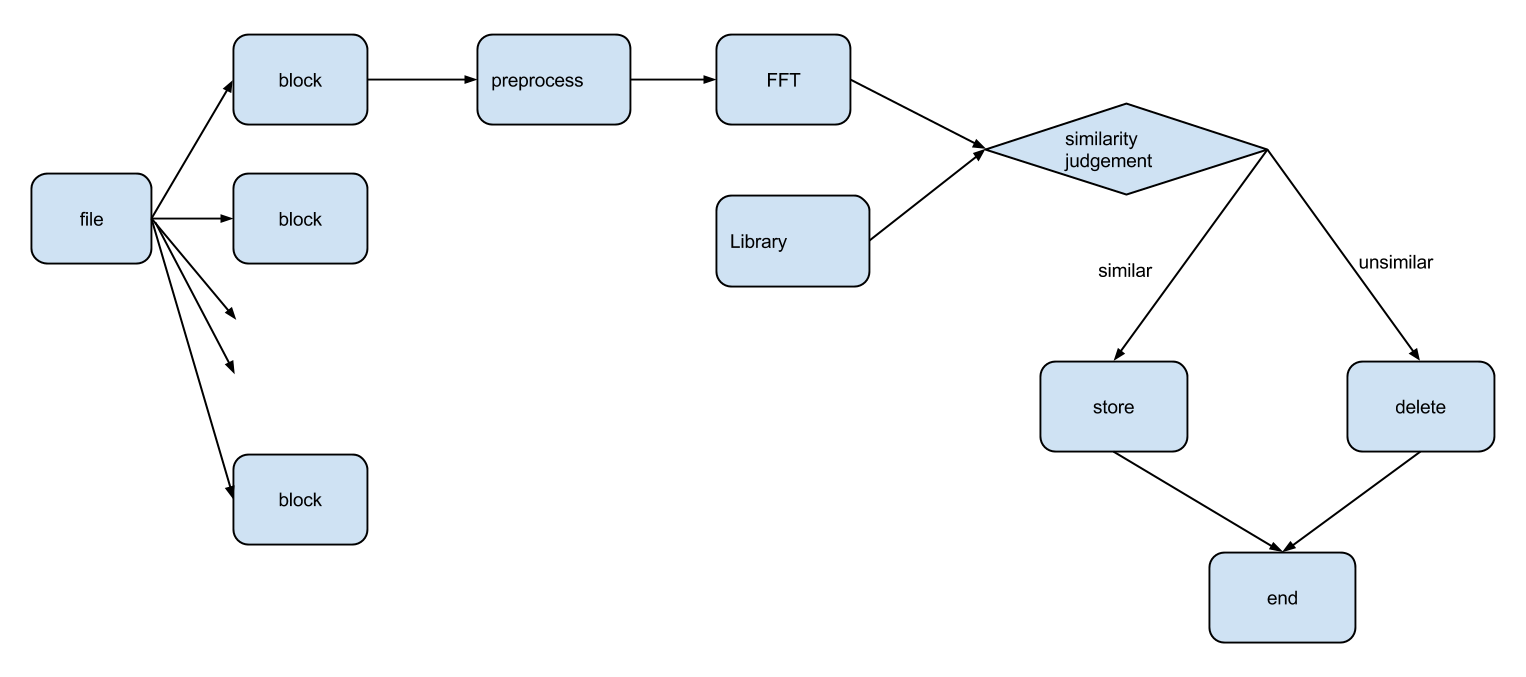
\includegraphics[origin=br,width=18cm]{chap4/archti.png}
    \bicaption[fig:archti]{这里将出现在插图索引}{基于FFT的文件去重算法架构.}{Fig}{Archtecture.}
    \end{minipage}     
\end{figure}

在图\ref{fig:archti}中,简单得描述了这个算法的简要步骤,首先,基于一些方法将一个大文件分成若干个文件块,这个文件块的输入将作为预处理的输出,预处理的输出将作为FFT的输入,FFT的输出是一个N维的向量,此时这个向量就代表了这个文件块,称为文件块的特征向量,与服务器端的库文件进行相似度的测试,此时需要依赖系统参数$\epsilon$,若相似,则不存储;若不相似,则存储,算法结束。本章节将详细介绍每一步骤的算法和设计理念。

\section{分块方法}
\label{sec:choice}

在第二章我们简单地提到过,若使用简单分块的方法,即对任意一个文件按照固定长度的切分成一个个文件块的方法,会遭受到插入问题(insertion problem)和删除问题(deletion problem)的影响导致去重性能急剧下降。简单来说,若采用简单分块的方法,那么边界是由预定义的分块大小决定的,此时如果任意插入或者删除一个字符,那么在这个分块之后的所有分块的内容都会向后或者向前偏移一个字符,导致了这个分块以后的所有分块都不相同,造成的结果是,即使后面的文件块毛无变化,但服务器上还是会存储多分冗余的拷贝。解决这个问题的一个方案是,不采用基于文件块大小作为块划分边界的依据,而是采用另外一种方法,即先定义一个滑动窗口,若文件的某一个滑动窗口满足一定事先约定的条件,那么这个滑动窗口对应的最后一个字节才是这个分块的最后一次字节。采用这种分块方法的好处的是,若随便插入或删除一个字符,那么只会影响当前块和之后的一个块,而其它块均不受影响,大大提高了存储的效率,此时的文件分块不再是以内容长度作为边界的依据值,还是根据内容。在本文基于FFT的文件去重算法中,我们采用简单分块的方式而不是基于滑动窗口的方法,理由主要是以下几点:

\begin{enumerate}
\item 保证了模型的简易性,将重点放在了FFT,余弦定理和系统参数$\epsilon$上
\item 在仿真阶段我们实现系统的主要框架,用简单分块大大简化了原形的实现
\item 本算法的重点并不是分块方法,可以由专门的论文来详细讨论
\end{enumerate}

事实上,若将此算法应用在工业界的实际使用中,那么考虑到存储的效率等等因素,一般还是会采用基于滑动窗口的分块方式,在之后的所有讨论中,将默认采用的时简单分块的大小,即直接将文件通过块的大小分成若干份,在服务器上的所有数据都是以块为单位,一个文件由若干个块组成。

\section{分块预处理}
\label{sec:proproc}

在本章中,将详细讲解分块预处理的必要性以及具体方法和步骤,我们将讨论一个现有的分块预处理的方法,分析这个方法的优缺点,并提出一种简单高效的分块方法。

\subsection{为什么要预处理}
\label{sec:why}

在\ref{fig:archti}中,我们可以看到,当文件分块以后,要经过一个预处理的过程,这一步是十分必要的,它的作用是将不同形式的输出和输入能够非常好地连接在一起,比如复数形式的FFT的输入是一个N维的复数向量,而一个分块是一个文件,它是一个个字节组成的数据,怎么接近无缝地连接这两个模块是十分重要的,在本文中,将详细讨论这个过程。

\subsection{预处理的方法}
\label{sec:appro}

在{参考}中,利用了离散傅里叶变换来解决网页去重,在这个算法中,把每个字符都映射成一个字符,那么每篇网页就可以表示成一个离散的序列$y(i)$,重复的网页应该具有相似的序列,对该序列进行离散傅里叶变换就可以得到傅里叶系数$a_n$和$b_n$,然后通过某种方法比较两个网页文件的傅里叶系数的前几项就可以大致比较出两个网页的相似度。在这篇研究中,预处理的方法主要是将一个字符映射到该字符对应的语义数值。

一个比较合适的字符到语义数值的转化应该满足,语义上相似的字符值对应的语义值应该相近,语义上不相似的字符值对应的语义值应该相差较大。该方法采用了如下方法作为计算每个字符的语义值的方法:以大量互联网上的文本素材作为基础,统计这些文本材料中字符和字符出现的关系,假设不同的字符数为N,那么统计的结果将是一个$N \times N$矩阵,其中$R(i, j)$的值定义为字符i和字符j相邻出现的次数除以字符i在文本素材中出现的总次数,若$i==j$,则这个值被定义为1,于是字符i的语义值就可以由N维向量$R(i)$来表示,但$R(i)$是一个向量,我们需要的是一个数值,也就是说需要对这个N维向量进行降维的操作,在该研究中采用K-L变换(Karhunen-Loeve)\upcite{vranic2001tools}的方法对$R(i)$降维,它是一种建立在统计特性基础上的一种转化,目的是将数据做转化,使得转化后数据的相关性最小。基于语义的预处理方法的优点是,这样的预处理方法比较新颖,并且是基于语义的,基于语义的一个最大的好处就是能够非常接近真实地反映原来数据之间的关系,并且能按照这样的关系模拟出一个具体的数值来代表这种关系,在某些基于语义的去重的场景下,这样的算法将非常合适。

实际上,对于互联网上的大数据而言,使用基于语义的预处理意义并不是特别大。首先,通常意义下的去重算法只关心两个文件严格意义上是否相同,即任意字符就代表文件的一个标志位,若这个字符不相同,则两个文件则不相同,而不在意这个字符与下一个字符之间的关系;其次,在上述的描述中我们需要实现构建一个$N \times N$的矩阵,这个矩阵是基于互联网上大量的文本素材所构建的,但是在实际中,这些素材的来源将很大程度上决定了这个$N \times N$矩阵的性质,需要严格保证这些素材的随机性,不仅如此,N将会是一个非常大的数字,表的一部分可能存在磁盘中,导致了一次读取表的操作都可能引起一次潜在的磁盘读取,对于高时效性高性能的大数据计算,这样的延时显然是不允许的。综上,基于语义的算法有很多不足之处,本文将提出一种简易的,可实现的同时具有保真性的预处理算法。

由分析可知,字符和字符之间的语义关系是不会影响两个文件之间相似度的判定,于是在本文中,将直接将文件的每一个字节看作是一个个离散的点,每个点取值范围为0至255,作为输入复数组中每一个复数的实数部分,即若一个1MB的文件经过预处理,则输出的是一个1*1024*1024维的复数向量,其中实部$real(i)=$第i字节对应的值,虚部$imag(i)=0$。这么做的好处有以下几点:

\begin{enumerate}
\item 完全脱离了语义的束缚,把着重点放在了每个字节上;
\item 从抽象角度上,更容易理解怎么把一个文件映射成一个离散的信号,以此作为FFT的输入;
\item 提高设计的简单性,实现的可行性。在仿真阶段,如果采用基于语义的预处理方法,将大大增加仿真的复杂度和难度,首先文本样本的选择是第一个问题,其次对于有些小型机器内存不一定能完全放下,这些在上面已讨论过。
\end{enumerate}

在下一小节说,将详细说明对变换后的文件使用傅里叶变换的意义和具体算法。

\section{对文本进行FFT变换的意义}
\label{sec:ffttr}

\subsection{文本作为离散的点}
从本质上来说,傅里叶变换不仅仅是一个数学工具,更是一种看待事物的一种思维方式,从时域上来讲,一切事物都在变化,换一个角度,若从频域上来讲,好像一切都是事先约定好的,有规律可循的,静止的。本章节将从抽象的角度来阐明怎么把FFT应用在文件去重这个领域上。

对于计算机而言,DFT是唯一能应用的一种傅里叶变换的变体,在数学的推导中,函数可以是连续的,所以有连续傅里叶变换和离散傅里叶变换,但计算机无法处理连续的信号,它只能对连续的信号进行采样,然后处理这些有间隔的离散的点。一个比较常用的例子是,音频信号在时域中显然是连续的,但计算机在记录音频并做处理的时候需要先对音频信号进行采样,两个样本之间会经历一个很小很小的时间$\Delta t$,于是整个音频的信号就可以变成时域上若干离散的点,从而可以进行下一步的处理。

理解傅里叶变换对输入转化的抽象意义是本文的一个难点,为了帮助读者理解对文本进行FFT变换的意义,将先举一个音乐的例子。在没有学习过乐器的人的理解中,音乐就是随时间变化的震动;而在一些乐器玩家的理解中,音乐是那些在乐谱上的音符。前者的理解是音乐在时域中的样子,而后者的理解是音乐在频域中的样子。在时域中,我们看到音乐随着琴键的上下按动而发出声音;在频域中,音乐是一些永恒的音符。对于任何一首乐曲,都可以通过不同琴键在不同的时间的敲击组成,其实本质上说的就是,任何周期函数,都可以看作是不同振幅不同频率不同相位的正弦波的叠加。

然后我们再来看离散的傅里叶变换,DFT的正向变换公式如下:$$X(k)=\frac{1}{N}\sum_{n=0}^{N-1}x(n)(\cos(\frac{2\pi kn}{N}) - j\sin(\frac{2\pi kn}{N}))$$可以很容易地看出,在频域上每一个点k对应的幅度值,都是由时域上所有点的加权和,而这个权重每个点都不一样,将欧拉等式应用于上式,我们可以得到$$X(k)=\frac{1}{N}\sum_{n=0}^{N-1}x(n)e^{-j2\pi kn/N}$$本文的一个难点是要理解将一个个分块的文件看成是一堆离散的信号,这是一种看待问题方式的创新和转变,也是傅里叶变换能够应用在很多领域(比如物理学、结构动力学、密码学等等)的一个重要原因,万事万物若从抽象的角度来看待均由一系列离散的点构成。我们将文件块经过预处理算法变成向量以后,对这个向量进行快速傅里叶变换,输出的这个N维向量可以看成是这个文件块的另外一种表达方式。在输出的N维向量中,每一个频率上的幅度值都由原来离散信号的所有点共同决定。

\subsection{FFT的必要性}

在上面的讨论中,我们看到,FFT的输入是一个N维的向量,输出也是一个N维的向量,那么为什么一定要经过FFT,直接用FFT的输入放到算法下一步的输入,即省去FFT这一步可以吗?答案是否定的。在下一节中,要解释这个问题需要先理解下一小节的内容,即我们是怎么处理和比较N维向量的,这是整个算法的最后的最后一步,两个N维向量若相似则说明找到重复,若不相似,说明这是一份新的文件块,服务器将存储文件块。在我们的算法中将定义两个变量$CHECK_UP$和$CHECK_DOWN$,若不进行FFT的变换,则会产生任意一个改变字符的权重全部加在了当前字符上,而我们希望这个字符的变化可以对整体的相似度的变化有影响,FFT非常好地完成了这项工作,每一个频率上的幅度都是由原来时域上的点加权得出。

\section{N维向量相似度的比较}
\label{sec:Nsimi}

\subsection{余弦定理的局限}

在现有技术中,比较N维向量相似度的一个主要的算法是余弦定理,这个算法非常容易理解,余弦定理算的时两个N维向量之间的夹角,若两个向量在坐标轴上靠得非常近,即之间的夹角非常小,那么我们就可以认为这两个向量是相似的向量。这个技术方法曾经被用在谷歌的新闻分类中,当时这个方法在分类领域的应用是一个非常大的创新点。本文算法设计的时候一开始也是将余弦定理为算法的输出比较,但是在写代码做实验的时候发现,余弦定理中有一个非常大的局限性,并且FFT的输出向量正好落在了这个局限性里头。

在上面的讨论中,我们谈到,在频域上任何一个点的幅度值都是由在时域上所有点加权的结果,那么有的点权重大有的点权重小,在加上文件本身对应的离散值的取值范围是0至255,同一个文件块的离散信号可能相差较大,这就导致了经过FFT变换以后维度和维度之间的数量级会相差特别大,下面的这幅图是应用基于FFT和余弦定理的算法的输出,其中$i$表示第几个点,$value$表示经过变换FFT变换以后的值。

\begin{lstlisting}[language={C}, caption={基于余弦定理检测相似度的结果}]
file "data_16_1" size is 16!
i = 0, value = 1162084.000000
i = 1, value = 31571.293828
i = 2, value = 9547.236365
i = 3, value = 4196.636560
i = 4, value = 1300.000000
i = 5, value = 12953.890439
i = 6, value = 10972.763635
i = 7, value = 8478.179173
i = 8, value = 20164.000000
i = 9, value = 8478.179173
i = 10, value = 10972.763635
i = 11, value = 12953.890439
i = 12, value = 1300.000000
i = 13, value = 4196.636560
i = 14, value = 9547.236365
i = 15, value = 31571.293828

file "data_16_2" size is 16!
i = 0, value = 1060900.000000
i = 1, value = 33937.760974
i = 2, value = 21162.751504
i = 3, value = 4277.091378
i = 4, value = 3412.000000
i = 5, value = 9801.435621
i = 6, value = 3581.248496
i = 7, value = 3039.712027
i = 8, value = 8836.000000
i = 9, value = 3039.712027
i = 10, value = 3581.248496
i = 11, value = 9801.435621
i = 12, value = 3412.000000
i = 13, value = 4277.091378
i = 14, value = 21162.751504
i = 15, value = 33937.760974
cos = 0.999735
\end{lstlisting}

在这个实验中,我们的两个文件分别是16字节,是两个完全不相似的文件。可以很明显看到第0个点的值的数量级远远大于别的维度值的数量级,导致的结果就是这一维的作用可能使别的维度效果非常非常小,于是这两个16维向量的夹角将非常地近,最后一行是两个向量的余弦值,可以看到夹角几乎为零。即对于两个不相似的文件,输出的结果是相似。

\subsection{一种新的方法}

事实证明,基于余弦定理的算法设计是有问题的,此时我们有两个选择:第一,改进现有的余弦算法,目的是让所有维度的值都在同意数量级内,因为不同维度的数据关系本来就不大,很难找到一种方法达到这样的目的;第二,设计一种新的算法,达到同样的目的。本文将采取第二种做法,设计一种新的做法来计算两个N维向量的相似度。算法的的代码如下:

\begin{lstlisting}[language={C}, caption={检测两个N维向量的相似度}]
int calc_simi(vector<double> &da, vector<double> &db, double &result)
{
    if (da.size() != db.size())
    {
        fprintf(stderr, "two vector size must be equal.\n");
        return THES_FAIL;
    }

    size_t vsize = da.size();
    int count = 0;
    for(size_t i=0; i < vsize; ++i)
    {
        double qt = da[i] / db[i];

        if (qt > CHECK_UP || qt < CHECK_DOWN)
            continue;

        count++;
    }
    
    result = double(count) / vsize;
    return THES_SUCC;
}
\end{lstlisting}
算法的输入是两个向量,分别放在两个vector里面,首先判断两个向量的长度是否一致,如果不一致,那么就错误,程序退出,文件在分块的时候就保证每个向量长度都是一致的,然后遍历这N维向量,定义一个上界CHECK\_UP和下界CHECK\_DOWN(这两个值可以用户自己配置以达到最佳效果),如果$da[i]$与$db[i]$的比值大于CHECK\_UP或者比值小于CHECK\_DOWN,那么就说明第i维度的两个值相差太远,视为无效维;否则,视为第i维度对整体的相似度有贡献,表现为将count加一,循环这个过程,直到全部处理完这两个N维向量,最后将count值除以向量的长度返回,这个值被我们定义为两个N维向量的相似度。

\subsection{可调节的相似度算法}

在这一节中,我们将定义一个系统参数$\epsilon$,取值范围$[0,1]$,来满足不同情况下对相似度的要求。我们定义,若两个文件的相似度大于$1-\epsilon$,那么这两个文件就是相同的文件。所以,这个值越大,就对相似性的要求越高。

从这个定义我们可以容易地得出,在两个极端的情况下,当$\epsilon$为0时,则只要任何一个字节不同,就被视为不同的文件;而当$\epsilon$为1时,则任何两个文件都会被视为相同的文件。所以这个参数的提出大大提高的算法应用场景的适应度,在传统的文件去重环境中,我们只要将这个系统参数设定为$0$即可。

这个系统参数的提出是个较新的做法,据我们有限的知识,以前还未在这个领域使用过类似的可配置的参数来调节不同场景对不同相似度的要求,这个参数具体影响的效果是使得查全率(正确去重数量 / 存在的重复)提高了,而使准确率(正确去重数量 / 存在的重复)下降了,所以正确地调节此值就非常重要。

\section{基于spark的算法设计}
\label{sec:spark}

在当下的大数据的环境下,spark已经受到了业界的一致好评,基于MapReduce的分布式计算方法也使得spark非常类似于Hadoop,保留的Hadoop优点的情况下,却又比Hadoop的通用性更加,迭代的运算效率更高,容错能力更强,所以在未来spark的发展前景可能会超越Hadoop,称为更通用的并行计算框架。在\cite{zaharia2012resilient}中,描述了RDD通用的架构,RDD是spark的基本构造模块,类似于分布式的不可变集。这些定义的操作如map或foreach,能很容易地并行处理;join运算,需要两个RDDs和一个共同建条目;规约的时候,通过用户指定基于键的函数来聚合条目。RDD从磁盘读取,然后为了提高之后的处理速度将数据都保存在内存中,也可以通过别的途径进行缓存,那样就可以不用每次都去读取他们,仅仅是这些基于提升磁盘速度的优化就比Hadoop块快了许多。当然,spark可能不会适应所有的场景,类似只更改很少条目的操作就不合适。原则上,就算只对一个条目修改,也必须对整个数据集备份。

在本章中,将设计一个并行算法,来执行我们的并行文件操作。在文件去重的领域,并行化是明显的趋势所在,除了第二章所提到的全文件检测算法以外,其它的算法均涉及到了文件分块的操作,所以这里有很多并行的工作可以做。

\begin{figure}[!h]
%\centering
    \begin{minipage}[b]{1\textwidth}
    \captionstyle{\centering}
    \centering
    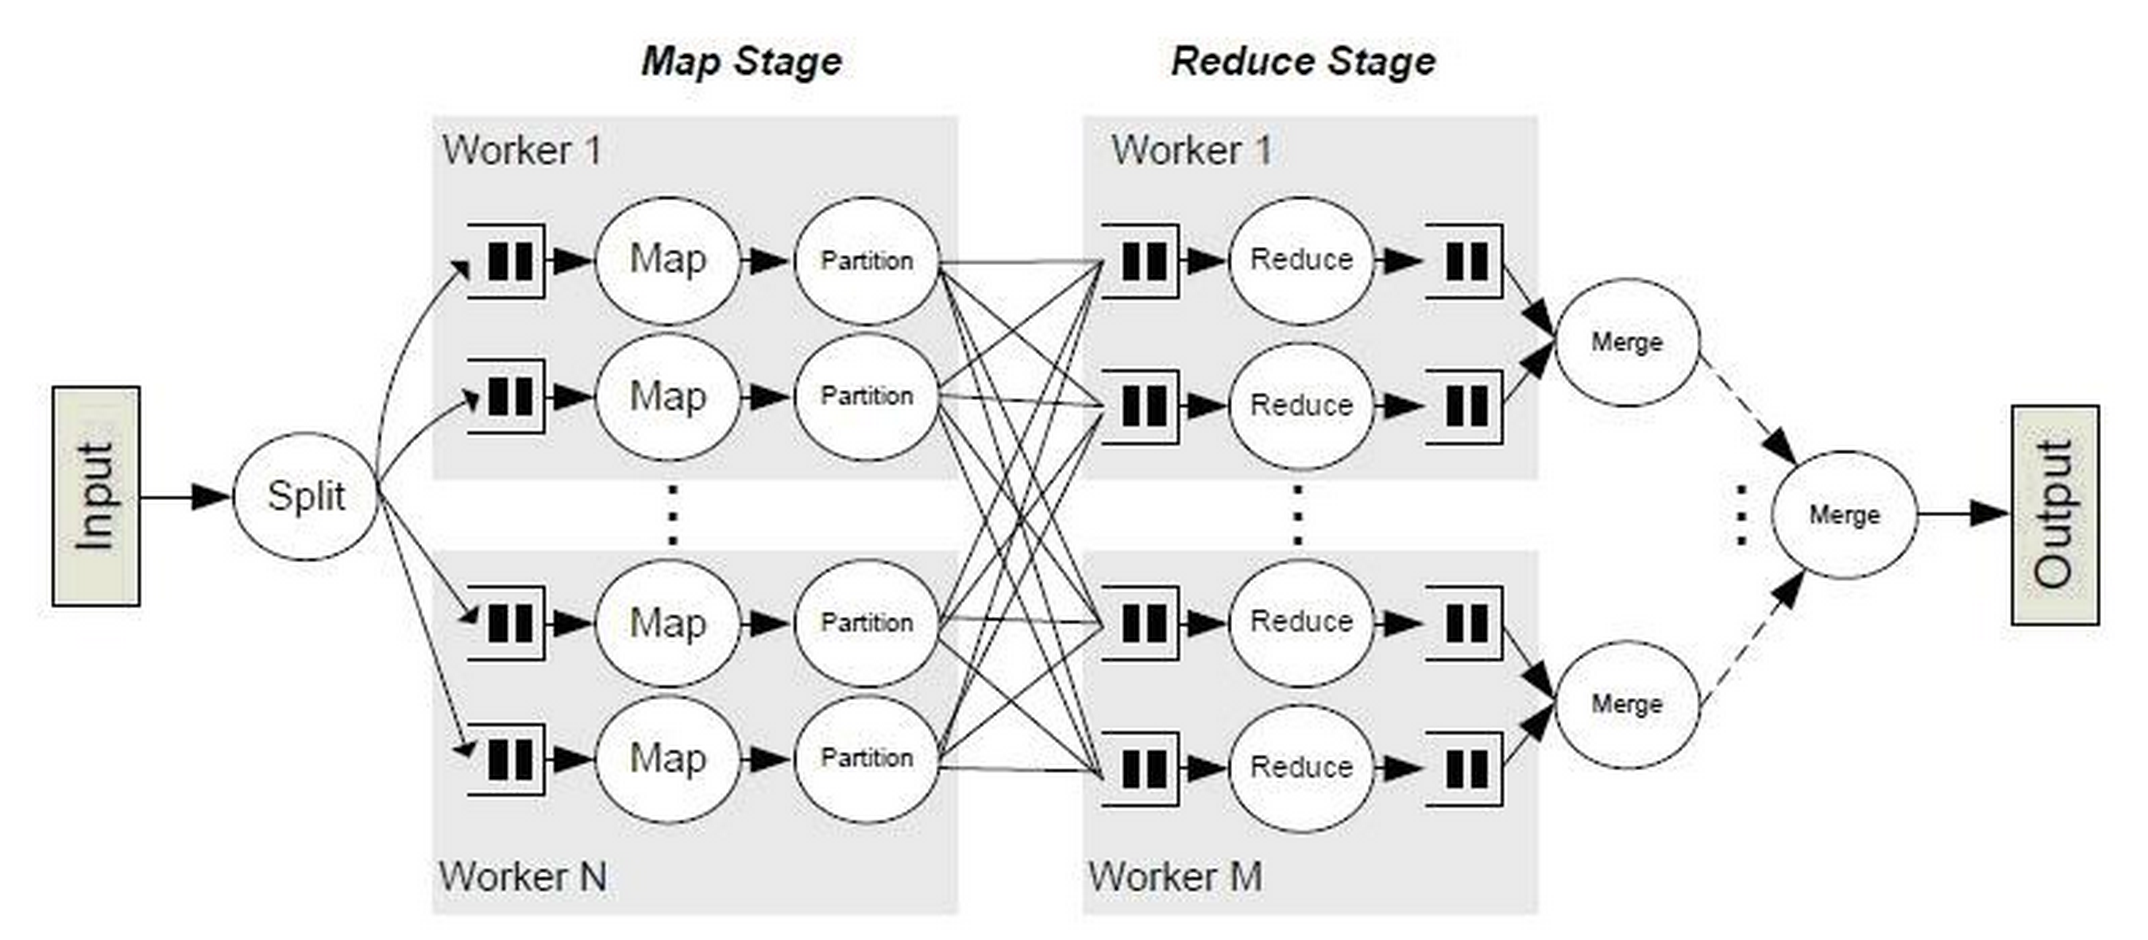
\includegraphics[origin=br,width=16cm]{chap4/sparkmapreduce.png}
    \bicaption[fig:sparkmr]{sparkMapReduce框架}{sparkMapReduce框架}{Fig}{sparkMapRedeuce Framework.}
    \end{minipage}     
\end{figure}

在图\ref{fig:sparkmr}中,显示了spark Map Reduce的通用框架图,首先将输入进行split操作,分成一块块可以并行操作的小块,之后进行map操作,输出进行partition分配到各自的reduce节点,reduce操作完了以后进行merge的操作,最后将结果输出。这个框架下最经典的一个例子是wordcount,计算一篇文章中每个单词出现的次数,用这个并行框架可以完美的结果,我们也将应用这个经典的框架在基于FFT的文件去重算法上,达到加速的目的。

用户的文件是一个大文件,我们将用户的文件拆分成小块,例如8MB或者16MB,这个值将由具体系统确定,那么在后台整个文件就可以由一个结构体来表示,结构体的一个成员是一个指向分块的指针数组,还原文件的时候只要遍历这个数组一次输出文件块的内容即可。下面我们将依次介绍Map Reduce框架中具体的细节:

\begin{enumerate}
    \item Split

        Split操作对应的是文件的分块操作,如果系统的文件块大小设定为16MB,那么用户输入一个1G文件时,这个文件将被分成64个文件块,于是系统将不再看到“大文件”这个概念,系统将看到的是64个固定文件块作为输入。将分成的这N个文件块分别塞入workers的队列中,等待worker读取进行下一步的Map操作。
    \item Map

        Map的输入是已经分好块的文件块,具体要做的是先对文件块做事先约定好的预处理,即把整个文件的字节值作为离散的点。然后进行快速傅里叶变换,此时的输出是一个N维的向量,这里的N等于文件块的大小。

    \item Partition

        Partition这一步将前面Map输出的N维向量分配到各个reduce节点,具体的分配方法有非常多,可参考现有的一些做法,一种比较普遍的方法是先讲N维向量降维成一维,然后哈希后取模作为reduce worker的序号。
    
    \item Reduce

        在reduce这一步与服务器上已有的文件进行比较,若发现满足任何在服务器上已有的快与这个块的相似度大于了$1-\epsilon$,那么就说明发现了重复的文件,那么保存一个指向相同文件块的指针即可;若与所有文件块的相似度都小于$1-\epsilon$,那么为这个文件块创建一片存储区域,服务器将存储这个文件块,并将指针指向这个新的文件块。

    \item Merge

        Merge的过程即是创建代表这个文件的结构体的过程,这个结构体里保存一个指针数组,这个数组的值由上一步Reduce产生,或指向新的文件块或指向旧的文件块。至此,一次上传文件的操作就完成了。
\end{enumerate}

在上述描述中,我们可以看到,若一个文件全部的文件块都是重复的,那么服务器上不用对存储这个文件做任何实质性的操作,只需要保存这个文件的元数据,即表示这个文件的结构体,也是会占用一部分系统资源,但是相比文件本身的大小,这个值可以忽略不计。

\section{小结}
\label{sec:conclusion}

在本章中,提出了基于FFT文件去重算法,首先介绍了算法的主要思想和具体框架,接着讨论了一些分块方法的优缺点和我们采用的方法以及选取的原因,我们又讨论了分块预处理这一过程,阐述了为什么要进行预处理以及一些现有的预处理方法和我们采用的方法;然后我们详细说明了对文本进行FFT变换的意义,包括将文本作为离散的点这种比较创新的思维方式,之后我们又讨论了进行FFT变换的必要性;我们又讨论了了两个N维向量相似度的比较算法,提出了余弦定理的局限性的同时提出了一种可调节系统参数$\eplison$的方法,最后,我们还设计了基于spark内存计算并行框架的算法实现。在下一章中,主要讨论我们实现的一个原形系统,从框架上实现了我们本文所提到的算法,并用一种用户友好的方式展现出来。

%%==========================
%% chapter01.tex for SJTU Master Thesis
%% based on CASthesis
%% modified by wei.jianwen@gmail.com
%% version: 0.3a
%% Encoding: UTF-8
%% last update: Dec 5th, 2010
%%==================================================

%\bibliographystyle{sjtu2} %[此处用于每章都生产参考文献]
\chapter{系统实现}
\label{chap:impl}

\section{xxx}
\label{sec:backgroud}

\section{小结}
\label{sec:cons}


%%==================================================
%% conclusion.tex for SJTU Master Thesis
%% based on CASthesis
%% modified by wei.jianwen@gmail.com
%% version: 0.3a
%% Encoding: UTF-8
%% last update: Dec 5th, 2010
%%==================================================

\chapter*{全文总结\markboth{全文总结}{}}
\addcontentsline{toc}{chapter}{全文总结}

这里是全文总结内容。

 %% 全文总结


%%%%%%%%%%%%%%%%%%%%%%%%%%%%%% 
%% 附录(章节编号重新计算,使用字母进行编号)
%%%%%%%%%%%%%%%%%%%%%%%%%%%%%% 
\appendix

% 附录中编号形式是"A-1"的样子
\renewcommand\theequation{\Alph{chapter}--\arabic{equation}}
\renewcommand\thefigure{\Alph{chapter}--\arabic{figure}}
\renewcommand\thetable{\Alph{chapter}--\arabic{table}}

%%%==================================================
%% app1.tex for SJTU Master Thesis
%% based on CASthesis
%% modified by wei.jianwen@gmail.com
%% version: 0.3a
%% Encoding: UTF-8
%% last update: Dec 5th, 2010
%%==================================================

\chapter{模板更新记录}
\label{chap:updatelog}

\textbf{2013年5月26日} v0.5.3发布,更正subsubsection格式错误,这个错误导致如"1.1 小结"这样的标题没有被正确加粗。

\textbf{2012年12月27日} v0.5.2发布,更正拼写错误:从``个人建立''更正为``个人简历''。在diss.tex加入ack.tex,更名后忘了引用。

\textbf{2012年12月21日} v0.5.1发布,在 \LaTeX 命令和中文字符之间留了空格,在Makefile中增加release功能。

\textbf{2012年12月5日} v0.5发布,修改说明文件的措辞,更正Makefile文件,使用metalog宏包替换xltxtra宏包,使用mathtools宏包替换amsmath宏包,移除了所有CJKtilde(\verb+~+)符号。

\textbf{2012年5月30日} v0.4发布,包含交大学士、硕士、博士学位论文模板。模板在\href{https://github.com/weijianwen/sjtu-thesis-template-latex}{github}上管理和更新。

\textbf{2010年12月5日} v0.3a发布,移植到 \XeTeX/\LaTeX 上。

\textbf{2009年12月25日} v0.2a发布,模板由CASthesis改名为sjtumaster。在diss.tex中可以方便地改变正文字号、切换但双面打印。增加了不编号的一章“全文总结”。
添加了可伸缩符号(等号、箭头)的例子,增加了长标题换行的例子。

\textbf{2009年11月20日} v0.1c发布,增加了Linux下使用ctex宏包的注意事项、.bib条目的规范要求,
修正了ctexbook与listings共同使用时的断页错误。

\textbf{2009年11月13日} v0.1b发布,完善了模板使用说明,增加了定理环境、并列子图、三线表格的例子。

\textbf{2009年11月12日} 上海交通大学硕士学位论文 \LaTeX 模板发布,版本0.1a。

 % 更新记录
%%% app2.tex for SJTU Master Thesis
%% based on CASthesis
%% modified by wei.jianwen@gmail.com
%% version: 0.3a
%% Encoding: UTF-8
%% last update: Dec 5th, 2010
%%==================================================

\chapter{Maxwell Equations}

选择二维情况,有如下的偏振矢量
\begin{subequations}
  \begin{eqnarray}
    {\bf E}&=&E_z(r,\theta)\hat{\bf z} \\
    {\bf H}&=&H_r(r,\theta))\hat{ \bf r}+H_\theta(r,\theta)\hat{\bm
      \theta}
  \end{eqnarray}
\end{subequations}
对上式求旋度
\begin{subequations}
  \begin{eqnarray}
    \nabla\times{\bf E}&=&\frac{1}{r}\frac{\partial E_z}{\partial\theta}{\hat{\bf r}}-\frac{\partial E_z}{\partial r}{\hat{\bm\theta}}\\
    \nabla\times{\bf H}&=&\left[\frac{1}{r}\frac{\partial}{\partial
        r}(rH_\theta)-\frac{1}{r}\frac{\partial
        H_r}{\partial\theta}\right]{\hat{\bf z}}
  \end{eqnarray}
\end{subequations}
因为在柱坐标系下,$\overline{\overline\mu}$是对角的,所以Maxwell方程组中电场$\bf
E$的旋度
\begin{subequations}
  \begin{eqnarray}
    &&\nabla\times{\bf E}=\mathbf{i}\omega{\bf B} \\
    &&\frac{1}{r}\frac{\partial E_z}{\partial\theta}{\hat{\bf
        r}}-\frac{\partial E_z}{\partial
      r}{\hat{\bm\theta}}=\mathbf{i}\omega\mu_rH_r{\hat{\bf r}}+\mathbf{i}\omega\mu_\theta
    H_\theta{\hat{\bm\theta}}
  \end{eqnarray}
\end{subequations}
所以$\bf H$的各个分量可以写为:
\begin{subequations}
  \begin{eqnarray}
    H_r=\frac{1}{\mathbf{i}\omega\mu_r}\frac{1}{r}\frac{\partial
      E_z}{\partial\theta } \\
    H_\theta=-\frac{1}{\mathbf{i}\omega\mu_\theta}\frac{\partial E_z}{\partial r}
  \end{eqnarray}
\end{subequations}
同样地,在柱坐标系下,$\overline{\overline\epsilon}$是对角的,所以Maxwell方程组中磁场$\bf
H$的旋度
\begin{subequations}
  \begin{eqnarray}
    &&\nabla\times{\bf H}=-\mathbf{i}\omega{\bf D}\\
    &&\left[\frac{1}{r}\frac{\partial}{\partial
        r}(rH_\theta)-\frac{1}{r}\frac{\partial
        H_r}{\partial\theta}\right]{\hat{\bf
        z}}=-\mathbf{i}\omega{\overline{\overline\epsilon}}{\bf
      E}=-\mathbf{i}\omega\epsilon_zE_z{\hat{\bf z}} \\
    &&\frac{1}{r}\frac{\partial}{\partial
      r}(rH_\theta)-\frac{1}{r}\frac{\partial
      H_r}{\partial\theta}=-\mathbf{i}\omega\epsilon_zE_z
  \end{eqnarray}
\end{subequations}
由此我们可以得到关于$E_z$的波函数方程:
\begin{eqnarray}
  \frac{1}{\mu_\theta\epsilon_z}\frac{1}{r}\frac{\partial}{\partial r}
  \left(r\frac{\partial E_z}{\partial r}\right)+
  \frac{1}{\mu_r\epsilon_z}\frac{1}{r^2}\frac{\partial^2E_z}{\partial\theta^2}
  +\omega^2 E_z=0
\end{eqnarray}
 % 麦克斯韦方程
% \include{body/app3}


%%%%%%%%%%%%%%%%%%%%%%%%%%%%%% 
%% 文后(无章节编号)
%%%%%%%%%%%%%%%%%%%%%%%%%%%%%% 
\backmatter

% 参考文献
% 使用 BibTeX
% 包含参考文献文件.bib
\bibliography{reference/chap1,reference/chap2,reference/chap3,reference/chap4,reference/chap5}

%% 个人简历(学士学位论文没有个人简历要求)
% %%==================================================
%% resume.tex for SJTU Master Thesis
%% based on CASthesis
%% modified by wei.jianwen@gmail.com
%% version: 0.3a
%% Encoding: UTF-8
%% last update: Dec 5th, 2010
%%==================================================

\begin{resume}

\begin{resumesection}{基本情况}
xxx,男,上海人,1985 年~12 月出生,未婚,
上海交通大学物理系在读博士研究生。
\end{resumesection}

\begin{resumelist}{教育状况}
XXXX 年~9 月至~XXXX 年~7 月,上海交通大学, 本科,专业:XXXX

XXXX 年~9 月至~XXXX 年~7 月,上海交通大学, 硕士研究生,专业:XXXX

XXXX 年~9 月至~XXXX 年~7 月,上海交通大学,
博士研究生(提前攻读博士),专业:XXXX
\end{resumelist}

\begin{resumelist}{工作经历}
无。
\end{resumelist}

\begin{resumelist}{研究兴趣}
XXXXXXX。
\end{resumelist}

\begin{resumelist}{联系方式}
通讯地址:上海市闵行区东川路800号,上海交通大学物理系

邮编:200240

E-mail: abcde@sjtu.edu.cn
\end{resumelist}

\end{resume}


% 致谢
%%==================================================
%% thanks.tex for SJTU Master Thesis
%% based on CASthesis
%% modified by wei.jianwen@gmail.com
%% version: 0.3a
%% Encoding: UTF-8
%% last update: Dec 5th, 2010
%%==================================================

\begin{thanks}

在论文定稿之际,心中颇多感慨。论文的写作过程是艰苦的,但我有幸得到了各位师、领导、同学、朋友、同事和亲人的教诲和帮助。没有他们,也就没有论文的最终成果。

首先我要特别感谢我的导师黄林鹏教授。本文是在黄老师的悉心指导下完成的。从本文的选题、构思、写作、修改直到最后定稿,都凝聚着导师的智慧、才华与心血。黄老师学识渊博、治学严谨求实、看待问题高屋建瓴、对待工作非常负责,为人随和坦诚,他的言传身教将使我终生受益。师恩难忘,在此,向黄老师表达我最诚挚的敬意与谢意!我还要感谢黄老师的博士生李素敏,每周都坚持和我讨论毕设的进展和阶段性成果,讨论算法的可行性和可实现性,并运用了多年写论文的经验帮我修改论文和提出意见,在此表示真诚的感谢。同时我还要感谢电子信息与电气工程学院的很多老师。从我入学至今,他们在有形无形中、有意无意中给予我很多知识,给我的选题、论证提供了诸多的启发与帮助。在此向这些老师以及给予我帮助的其他老师表示诚挚的感谢。我还要感谢我的同窗同学,他们在论文写作过程中给予了我很多的帮助。

最后我还要感谢我的家人,感谢他们给予我生活和精神上的关心、支持和鼓励,才能毫无后顾之忧的学习。

值此论文完成之际,我谨向以上曾经给予我指导和关心的老师、同学、同事和家人意最诚挚的谢意!

\end{thanks}


% 发表文章目录
%%%==================================================
%% pub.tex for SJTU Master Thesis
%% based on CASthesis
%% modified by wei.jianwen@gmail.com
%% version: 0.3a
%% Encoding: UTF-8
%% last update: Dec 5th, 2010
%%==================================================

\begin{publications}{99}

    \item\textsc{Chen H, Chan C~T}. {Acoustic cloaking in three dimensions using acoustic metamaterials}[J].
      Applied Physics Letters, 2007, 91:183518.

    \item\textsc{Chen H, Wu B~I, Zhang B}, et al. {Electromagnetic Wave Interactions with a Metamaterial Cloak}[J].
      Physical Review Letters, 2007, 99(6):63903.
    
\end{publications}


% 参与项目列表
%%%==================================================
%% projects.tex for SJTU Master Thesis
%% based on CASthesis
%% modified by wei.jianwen@gmail.com
%% version: 0.3a
%% Encoding: UTF-8
%% last update: Dec 5th, 2010
%%==================================================

\begin{projects}{99}

    \item 973项目“XXX”
    \item 自然基金项目“XXX”
    \item 国防项目“XXX”
    
\end{projects}


\end{document}
